\section{课程综述}

回归分析是一类重要的监督学习算法,主要用于预测连续型目标变量。其核心思想是建立特征变量与目标变量之间的映射关系,广泛应用于经济预测、医学研究、工程控制等领域。
\subsection{课题简介}
在机器学习研究领域中,传统回归算法(如最小二乘线性回归、岭回归、Lasso、Elastic Net 等)以参数可解释性强、样本效率高与训练稳定为主要优势,被广泛用于连续变量预测与因果线索探索。其核心思想是基于明确的函数假设与正则化约束,最小化经验风险并抑制过拟合。本项目基于Ridge Net构建回归模型,采用K折交叉验证 进行选参,并以MSE/MAE在独立测试集评估性能。
\subsection{课题目标}
课题的目标为对于目标数据集"Boston House Prices”,搭建相应的传统机器学习回归模型,完成用房屋的多维属性预测最终售价,并能取得较优的性能。整个实验课题包含数据准备、数据预处理、模型搭建、模型训练、模型优化、模型检测、实验总结等过程。
\subsection{线性回归的历史发展}

线性回归作为最古老、最基础的回归方法,其历史可以追溯到19世纪初:

\begin{itemize}
    \item \textbf{1805年}:法国数学家勒让德(Adrien-Marie Legendre)首次发表最小二乘法
    \item \textbf{1809年}:德国数学家高斯(Carl Friedrich Gauss)独立提出并完善了最小二乘理论
    \item \textbf{1885年}:英国统计学家高尔顿(Francis Galton)在研究遗传问题时首次使用"回归"一词
    \item \textbf{20世纪}:费希尔(Ronald Fisher)等统计学家建立了线性回归的现代理论基础
\end{itemize}

线性回归的发展历程体现了从数学理论到实际应用的完整链条,至今仍在机器学习和统计学中占据重要地位。

\subsection{常见回归算法}

\begin{itemize}
    \item \textbf{线性回归}:通过线性函数$y = \beta_0 + \beta_1x_1 + \cdots + \beta_nx_n + \epsilon$拟合数据,最小化残差平方和
    \item \textbf{岭回归}:在线性回归基础上加入L2正则化项$\lambda\sum_{i=1}^n\beta_i^2$,防止过拟合
    \item \textbf{Lasso回归}:使用L1正则化$\lambda\sum_{i=1}^n|\beta_i|$,能够产生稀疏解,实现特征选择
\end{itemize}

\subsection{线性回归应用实例}

线性回归在实际中有广泛的应用,以下是一些典型实例:

\textbf{房价预测}:
\begin{itemize}
    \item 使用房屋面积、卧室数量、地理位置等特征预测房价
    \item 模型形式:$\text{价格} = \beta_0 + \beta_1\times\text{面积} + \beta_2\times\text{卧室数} + \cdots$
\end{itemize}
\begin{figure}[!htb]
	\centering
	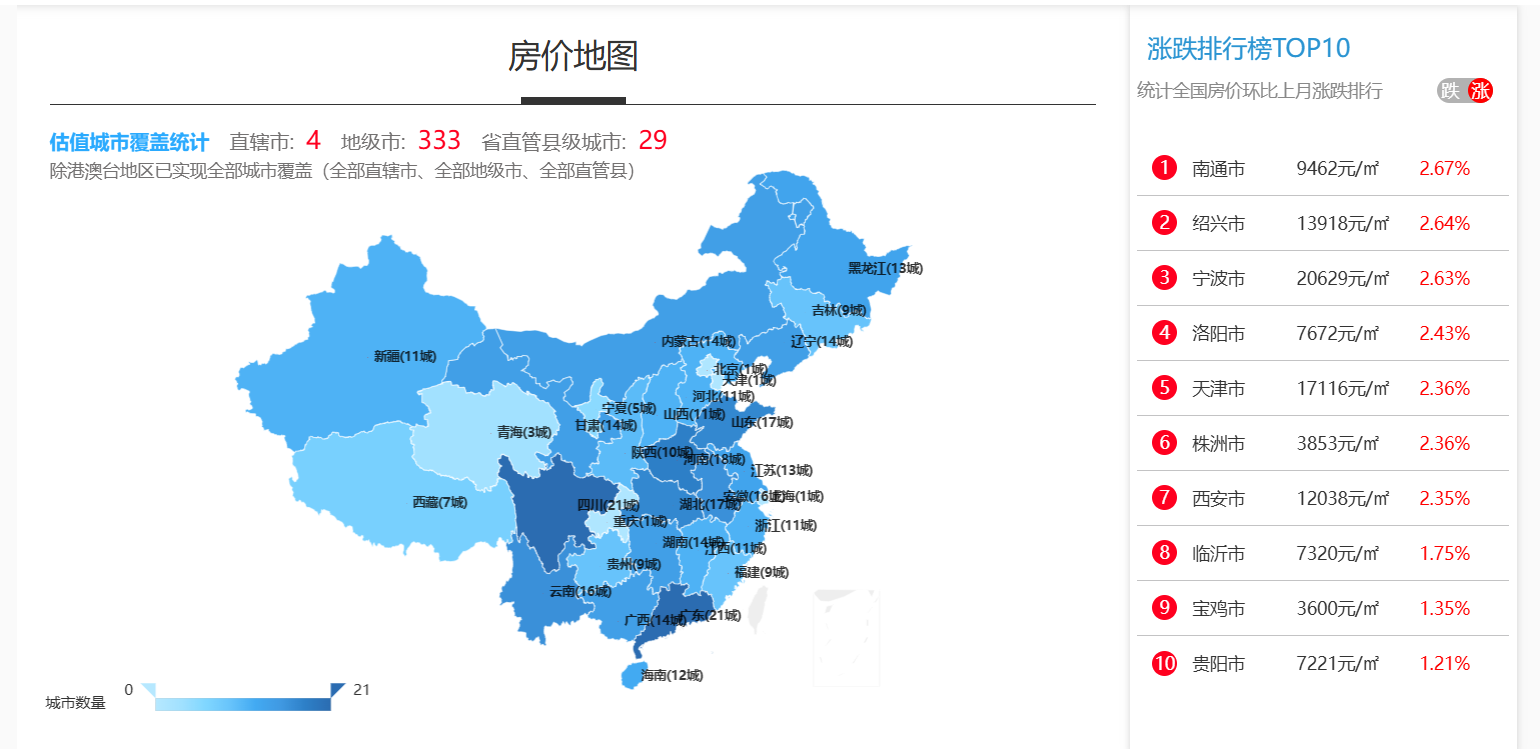
\includegraphics[width=0.70\textwidth]{./figures/house.png}
	\caption{房价地图}
\end{figure}

\textbf{医学研究}:
\begin{itemize}
    \item 基于患者年龄、体重、生活习惯等预测血压水平
    \item 分析药物剂量与治疗效果的关系
\end{itemize}

\textbf{网点数据分析}:
\begin{itemize}
    \item 分析不同平台对于电商销售额的影响。
\end{itemize}



\subsection{模型评估}

回归模型常用评估指标包括:
\begin{itemize}
    \item \textbf{均方误差(MSE)}:$\frac{1}{n}\sum_{i=1}^n(y_i - \hat{y}_i)^2$
    \item \textbf{均方根误差(RMSE)}:$\sqrt{\text{MSE}}$
    \item \textbf{平均绝对误差(MAE)}:$\frac{1}{n}\sum_{i=1}^n|y_i - \hat{y}_i|$
    \item \textbf{决定系数($R^2$)}:$1 - \frac{\sum_{i=1}^n(y_i - \hat{y}_i)^2}{\sum_{i=1}^n(y_i - \bar{y})^2}$
\end{itemize}

随着大数据时代的发展,回归分析在推荐系统、风险评估、量化投资等新兴领域继续发挥着重要作用。
\subsection{数据集选取}
基于以上的场景应用,我们选择了三个数据集用以训练自己的模型。
\subsubsection{波士顿房价数据集(Boston House Price Dataset)}
该数据集来源于\texttt{https://huggingface.co/datasets/mrseba/boston\_house\_price},是机器学习回归任务的经典基准数据集,源于1970年代美国波士顿地区住房市场普查,共包含506条样本,核心目标是通过12个输入属性预测街区的房价中位数(MEDV,单位:千美元),为房地产市场分析与区域经济研究提供数据支撑。

其12个输入属性涵盖社会、经济、环境等多维度信息,各变量详情如下表所示:

\begin{table}[!hpt]
  \caption{波士顿房价数据集特征变量详情}
  \label{tab:boston_house_features}
  \centering
  \small
  % 用p{宽度}固定列宽,总宽度控制在文本宽度内,行内自动换行
  \begin{tabular}{@{}p{0.12\textwidth}p{0.25\textwidth}p{0.18\textwidth}p{0.4\textwidth}@{}} \toprule
    \textbf{特征名称} & \textbf{变量含义} & \textbf{数据类型} & \textbf{对房价(MEDV)的影响逻辑} \\ \midrule
    CRIM & 街区人均犯罪率 & 连续型(数值) & 负相关:犯罪率越高,居住安全性越低,房价通常越低 \\
    ZN & 占地面积超过25000平方英尺的住宅用地比例 & 连续型(数值) & 正相关:大户型住宅占比高,区域居住品质偏高,房价更高 \\
    INDUS & 街区非零售商业用地比例(英亩/城镇) & 连续型(数值) & 负相关:商业用地密集可能导致居住环境嘈杂,降低居住舒适度 \\
    CHAS & 查尔斯河虚拟变量(1=临近河流,0=不临近) & 离散型(二分类) & 正相关:临水地段通常具备景观优势,房价存在“临水溢价” \\
    NOX & 一氧化氮浓度(百万分之一) & 连续型(数值) & 负相关:污染物浓度高代表环境质量差,对房价有抑制作用 \\
    RM & 每栋住宅的平均房间数 & 连续型(数值) & 强正相关:房间数越多,住宅实用面积与居住空间越大,房价显著更高 \\
    AGE & 1940年之前建成的自住单位比例 & 连续型(数值) & 负相关:房龄越长,房屋设施老化程度越高,维护成本增加,房价偏低 \\
    DIS & 到波士顿5个就业中心的加权距离 & 连续型(数值) & 负相关:距离就业中心越近,通勤便利性越强,房价越高 \\
    RAD & 到高速公路的可达性指数(指数越高可达性越好) & 连续型(数值) & 正相关:交通便利性提升居住便捷度,对房价有正向拉动 \\
    TAX & 每10000美元房产的全额财产税率 & 连续型(数值) & 负相关:税率越高,持有房产的成本越高,可能降低房价吸引力 \\
    PTRATIO & 街区师生比(学生数/教师数) & 连续型(数值) & 负相关:师生比越低(教师资源越充足),教育配套越好,房价越高 \\ \bottomrule
  \end{tabular}
\end{table}


\subsubsection{个人医疗费用数据集(Insurance Dataset)}
该数据集来源于\texttt{https://www.kaggle.com/datasets/mirichoi0218/insurance},是个性化风险预测与回归分析的典型数据集,采集自真实个人医疗保险记录,共1338条样本,核心任务是根据个人基本信息与健康状况,预测年度医疗费用(insuranceclaim),适用于保险公司保费定价、医疗成本核算场景。

数据集变量分为数值型与字符串型(需编码处理),各变量详情如下表所示:

\begin{table}[!hpt]
  \caption{个人医疗费用数据集变量详情}
  \label{tab:insurance_variables}
  \centering
  \small
  \begin{tabular}{@{}p{0.12\textwidth}p{0.2\textwidth}p{0.18\textwidth}p{0.22\textwidth}p{0.23\textwidth}@{}} \toprule
    \textbf{变量名称} & \textbf{变量含义} & \textbf{数据类型} & \textbf{取值范围/类别} & \textbf{对医疗费用的潜在影响} \\ \midrule
    age & 被保险人年龄 & 数值型(连续) & 18-64岁 & 正相关:年龄增长导致慢性病风险升高,医疗需求增加 \\
    sex & 性别 & 字符串型(分类) & "male"(男性)、"female"(女性) & 差异较小:女性可能因生育、妇科疾病产生特定费用 \\
    bmi & 体重指数(Body Mass Index) & 数值型(连续) & 15.96-53.13 & 正相关:BMI异常增加健康风险,如肥胖与糖尿病相关 \\
    children & 被保险人子女数量 & 数值型(离散) & 0-5人 & 正相关:子女数量越多,家庭整体医疗需求越高 \\
    smoker & 是否吸烟 & 字符串型(分类) & "yes"(吸烟)、"no"(不吸烟) & 强正相关:吸烟与重疾相关,医疗费用显著更高 \\
    region & 居住区域 & 字符串型(分类) & "northeast"等4个区域 & 区域差异:医疗资源、病种流行率不同导致费用差异 \\
    charges & 年度医疗费用(目标变量) & 数值型(连续) & 1121.87-63770.43美元 & - \\ \bottomrule
  \end{tabular}
\end{table}

字符串变量需针对性编码:二分类变量(sex、smoker)可采用标签编码(如male→1、female→0;yes→1、no→0),避免独热编码的特征冗余;多分类变量(region)推荐独热编码(转换为4个二进制特征),或目标编码(用区域内charges均值编码,需交叉验证防过拟合)。

\subsubsection{网店销售额预测数据集(Advertising Simple Dataset)}
该数据集来源于\texttt{https://www.kaggle.com/datasets/tohuangjia/advertising-simple-dataset},是营销效果分析与回归预测的简化数据集,共200条样本。通过记录网店不同渠道广告费用,预测同期产品销售额,适用于电商广告预算分配、营销效果评估场景。

数据集变量设计简洁,均为数值型,无需复杂的分类变量编码,各变量详情如下表所示:

\begin{table}[!hpt]
  \caption{网店销售额预测数据集变量详情}
  \label{tab:advertising_variables}
  \centering
  \small
  \begin{tabular}{@{}p{0.15\textwidth}p{0.22\textwidth}p{0.18\textwidth}p{0.25\textwidth}p{0.17\textwidth}@{}} \toprule
    \textbf{变量名称} & \textbf{变量含义} & \textbf{数据类型} & \textbf{取值范围(单位:千美元)} & \textbf{对销售额的影响逻辑} \\ \midrule
    TV & 电视广告投放费用 & 连续型 & 0.7-296.4 & 正相关:覆盖人群广,品牌曝光度高,拉动作用最强 \\
    Radio & 广播广告投放费用 & 连续型 & 0.0-49.6 & 正相关:针对特定场景,覆盖精准度较高,影响范围小于电视 \\
    Newspaper & 报纸广告投放费用 & 连续型 & 0.3-114.0 & 弱正相关/无显著相关:时效性强但留存率低,转化效果弱 \\
    Sales & 同期产品销售额(目标变量) & 连续型 & 1.6-27.0 & - \\ \bottomrule
  \end{tabular}
\end{table}
\subsubsection{代码说明}
\begin{lstlisting}[
  language=Python,         % 指定语法高亮的编程语言
  caption={下载数据集},
  label=lst:download,
  frame=single,            % 添加单线边框
  basicstyle=\small\ttfamily, % 设置字体为等宽小号字体
  numbers=left,            % 显示行号
  numberstyle=\tiny,       % 行号使用极小字体
  backgroundcolor=\color{bg}, % 设置背景色
  commentstyle=\color{commentcolor}\itshape, % 注释样式
  keywordstyle=\color{keywordcolor}\bfseries, % 关键字样式
  stringstyle=\color{stringcolor}, % 字符串样式
  breaklines=true,         % 允许自动换行
  showstringspaces=false   % 不显示字符串中的空格
]
y_label="MEDV"
_target_path="./dataset"
data_path=_target_path+"/train.csv"
title="波士顿房价数据集"
def download_dataset_boston():
	ds = load_dataset("mrseba/boston_house_price")
	ds.save_to_disk("./dataset")
	train_df = ds['train'].to_pandas()
	train_df.to_csv("./dataset/train.csv", index=False)
	print("Dataset downloaded and saved to disk.")
if __name__ == '__main__':
	download_dataset_boston()
\end{lstlisting}


\par 通过设置download.py当中的描述数据集信息的设置,可以做到对于任何一个线性回归数据集的适应。限制条件是不允许使用字符描述的列值,以及数据集必须以csv格式保存。对于每个变量说明如下:
\begin{itemize}
\item \bf{y\_label}:这个csv当中的y标签对应的列名。
\item \bf{\_target\_path}:数据集的csv文件存储的url
\item \bf{data\_path}:数据在本地存储的相对位置
\item \bf{title}:希望以什么样的名字命名这个回归图像
\end{itemize}

\par 设置好之后下载数据集 python download.py 再运行python main.py 即可开始回归


